%%%%%%%%%%%%%%%%%%%%%%%%%%%%%%%%%%%%%%%%%
% Beamer Presentation
% LaTeX Template
% Version 1.0 (10/11/12)
%
% This template has been downloaded from:
% http://www.LaTeXTemplates.com
%
% License:
% CC BY-NC-SA 3.0 (http://creativecommons.org/licenses/by-nc-sa/3.0/)
%
%%%%%%%%%%%%%%%%%%%%%%%%%%%%%%%%%%%%%%%%%

%----------------------------------------------------------------------------------------
%	PACKAGES AND THEMES
%----------------------------------------------------------------------------------------

\documentclass{beamer}

\mode<presentation> {

% The Beamer class comes with a number of default slide themes
% which change the colors and layouts of slides. Below this is a list
% of all the themes, uncomment each in turn to see what they look like.

%\usetheme{default}
%\usetheme{AnnArbor}
%\usetheme{Antibes}
%\usetheme{Bergen}
%\usetheme{Berkeley}
%\usetheme{Berlin}
%\usetheme{Boadilla}
%\usetheme{CambridgeUS}
%\usetheme{Copenhagen}
%\usetheme{Darmstadt}
%\usetheme{Dresden}
%\usetheme{Frankfurt}
%\usetheme{Goettingen}
%\usetheme{Hannover}
%\usetheme{Ilmenau}
%\usetheme{JuanLesPins}
%\usetheme{Luebeck}
\usetheme{Madrid}
%\usetheme{Malmoe}
%\usetheme{Marburg}
%\usetheme{Montpellier}
%\usetheme{PaloAlto}
%\usetheme{Pittsburgh}
%\usetheme{Rochester}
%\usetheme{Singapore}
%\usetheme{Szeged}
%\usetheme{Warsaw}

% As well as themes, the Beamer class has a number of color themes
% for any slide theme. Uncomment each of these in turn to see how it
% changes the colors of your current slide theme.

%\usecolortheme{albatross}
\usecolortheme{beaver}
%\usecolortheme{beetle}
%\usecolortheme{crane}
%\usecolortheme{dolphin}
%\usecolortheme{dove}
%\usecolortheme{fly}
%\usecolortheme{lily}
%\usecolortheme{orchid}
%\usecolortheme{rose}
%\usecolortheme{seagull}
%\usecolortheme{seahorse}
%\usecolortheme{whale}
%\usecolortheme{wolverine}

%\setbeamertemplate{footline} % To remove the footer line in all slides uncomment this line
%\setbeamertemplate{footline}[page number] % To replace the footer line in all slides with a simple slide count uncomment this line

%\setbeamertemplate{navigation symbols}{} % To remove the navigation symbols from the bottom of all slides uncomment this line

\setbeamertemplate{frametitle}[default][center]
}

\usepackage{graphicx} % Allows including images
\usepackage{booktabs} % Allows the use of \toprule, \midrule and \bottomrule in tables
\usepackage{multimedia}
%\usepackage{movie15}
\usepackage{caption}
\usepackage{subcaption}
\usepackage{amsfonts}
\usepackage{epstopdf}
\usepackage{bigints}
\usepackage{amsmath}
\usepackage{hyperref}
\usepackage{verbatim}
\usepackage{mathrsfs}
\usepackage{color}
\usepackage[outline]{contour}
\usepackage{multirow}

\contourlength{1pt}

\newcommand\Bo{\mbox{\textit{Bo}}}  % Bond number
\newcommand\Rey{\mbox{\textit{Re}}}  % Reynolds number
\newcommand\Ri{\mbox{\textit{Ri}}}  % Richardson number

\def\Xint#1{\mathchoice
{\XXint\displaystyle\textstyle{#1}}%
{\XXint\textstyle\scriptstyle{#1}}%
{\XXint\scriptstyle\scriptscriptstyle{#1}}%
{\XXint\scriptscriptstyle\scriptscriptstyle{#1}}%
\!\int}
\def\XXint#1#2#3{{\setbox0=\hbox{$#1{#2#3}{\int}$}
\vcenter{\hbox{$#2#3$}}\kern-.5\wd0}}
\def\ddashint{\Xint=}
\def\dashint{\Xint-}

%----------------------------------------------------------------------------------------
%	TITLE PAGE
%----------------------------------------------------------------------------------------

\title[Modeling volcanic processes]{Gravity currents in volcanology} % The short title appears at the bottom of every slide, the full title is only on the title page

\author[Paul Jarvis]{Paul A. Jarvis} % Your name
\institute[UNIGE] % Your institution as it will appear on the bottom of every slide, may be shorthand to save space
{
\textit{paul.jarvis@unige.ch} % Your email address
}
\date{22nd November 2019} % Date, can be changed to a custom date
\begin{columns}

  \begin{column}{0.33\paperwidth}
    $$\includegraphics[width=0.3\paperwidth]{UNIGE_logo.jpg}$$
  \end{column}

  \begin{column}{0.33\paperwidth}
    $$\includegraphics[width=0.3\paperwidth]{redoubt.jpg}$$
  \end{column}

  \begin{column}{0.33\paperwidth}
    $$\includegraphics[width=0.3\paperwidth]{etna.jpg}$$
  \end{column}
  
\end{columns}
\vspace{-2cm}

\DeclareMathOperator\erf{erf}

\begin{document}

\begin{frame}
\titlepage % Print the title page as the first slide
\end{frame}

%\begin{frame}
%\frametitle{Overview} % Table of contents slide, comment this block out to remove it
%\tableofcontents % Throughout your presentation, if you choose to use \section{} and \subsection{} commands, these will automatically be printed on this slide as an overview of your presentation
%\end{frame}


%----------------------------------------------------------------------------------------
%	PRESENTATION SLIDES
%----------------------------------------------------------------------------------------

%------------------------------------------------
%\section{First Section} % Sections can be created in order to organize your presentation into discrete blocks, all sections and subsections are automatically printed in the table of contents as an overview of the talk
%------------------------------------------------

%\subsection{Subsection Example} % A subsection can be created just before a set of slides with a common theme to further break down your presentation into chunks

\begin{frame}
  \frametitle{Lava flows - Flow on a slope}

  Consider flow of a viscous fluid on a slope \\

  \begin{columns}[t]

    \begin{column}{0.5\paperwidth}

      $$\includegraphics[width=0.3\paperwidth]{slope_flow.png}$$

    \end{column}

    \begin{column}{0.5\paperwidth}

      Want to determine shear stress at base of flow \\

      \vspace{1cm}
      
      \textbf{Shear stress} = Force per unit area extered on ground \\
    \end{column}
    
  \end{columns}
  
\end{frame}
%-----------------------------------------------
\begin{frame}
  \frametitle{Lava flows - Flow on a slope}

  \begin{columns}[t]

    \begin{column}{0.5\paperwidth}

      $$\includegraphics[width=0.3\paperwidth]{slope_flow_vol.png}$$

      $$ h' = \frac{h}{\cos\theta} $$

      $$ W = \frac{\rho h x' d g}{\cos \theta}$$
    \end{column}

    \begin{column}{0.5\paperwidth}

      Consider a volume of a thin slice

      $$ V = h' x' d $$

      where $d$ = width of flow \\

      So, total weight of column:

      $$ W = \rho V g = \rho h' x' d g $$

      \vspace{-0.5cm}
      $$\includegraphics[width=0.3\paperwidth]{slope_trig.png}$$
    \end{column}
    
  \end{columns}
  
\end{frame}
%-----------------------------------------------
\begin{frame}
  \frametitle{Lava flows - Flow on a slope}

  \begin{columns}[t]

    \begin{column}{0.5\paperwidth}

      $$\includegraphics[width=0.3\paperwidth]{slope_flow_weight.png}$$

      Area under column $A = X d = \frac{x' d}{\cos \theta}$

      Shear stress:

      $$ \tau = \frac{W'}{A} = \rho g h \sin \theta $$
    \end{column}

    \begin{column}{0.5\paperwidth}

      Downslope component of weight:

      $$ W' = W \sin \theta $$

      $$ W' = \frac{\rho h x' d g \sin \theta}{\cos \theta}$$

      $$\includegraphics[width=0.3\paperwidth]{slope_flow_area.png}$$
      
    \end{column}
    
  \end{columns}
  
\end{frame}
%-----------------------------------------------
\begin{frame}
  \frametitle{Lava flow rheology}

  \begin{columns}[t]

    \begin{column}{0.5\paperwidth}

      $$\includegraphics[width=\textwidth]{flow_curves.pdf}$$

    \end{column}

    \begin{column}{0.5\paperwidth}

      Crystal-free lavas behave as Newtonian fluids \\

      \vspace{1cm}

      Partially crystallised lavas have a yield stress $\tau_{0}$ \\

      \vspace{1cm}

      Lavas have a minimum thickness below which they cannot flow:

      $$ h_{0} = \frac{\tau_{0}}{\rho g \sin \theta}$$

      This thickness depends on the topography \\
    \end{column}
    
  \end{columns}
  
\end{frame}
%-----------------------------------------------
\begin{frame}
  \frametitle{Jeffrey's model for lava flow velocity}

  \begin{columns}[t]

    \begin{column}{0.5\paperwidth}

      $$\includegraphics[width=\textwidth]{slope_vel.png}$$

    \end{column}

    \begin{column}{0.5\paperwidth}

      Mean velocity inside a channel:

      $$ \bar{u} = \frac{h^{2} \rho g \sin \theta}{B \eta} $$

      $B$ = constant depending on channel geometry \\

      \vspace{1cm}
      
      Expression is valid for a Newtonian lava \\

      \vspace{1cm}
      
      More complicated models for Bingham fluids \\

    \end{column}
    
  \end{columns}
  
\end{frame}
%-----------------------------------------------
\begin{frame}
  \frametitle{Controls on lava flow}

  Lava flow rates depend on:

  \begin{columns}[t]

    \begin{column}{0.5\paperwidth}

      \begin{itemize}
      \item Topography \\
        \begin{itemize}
        \item Slope angle \\
        \item Channel geometry (if it exists) \\
        \end{itemize}
      \end{itemize}

    \end{column}

    \begin{column}{0.5\paperwidth}

    \begin{itemize}
    \item Rheology \\
      \begin{itemize}
      \item Viscosity \\
      \item Yield stress \\ 
      \end{itemize}
    \end{itemize}

  \end{column}

\end{columns}

  \vspace{0.5cm}
  
  Rheology is most difficult to assess - it depends on:

  \begin{columns}[t]

    \begin{column}{0.5\paperwidth}

      \begin{itemize}
      \item Composition \\
      \item \textbf{Temperature} \\
      \item Crystallinity \\
      \item Vesivularity \\
      \end{itemize}

    \end{column}

    \begin{column}{0.5\paperwidth}

      \vspace{-1cm}
      
      $$\includegraphics[width=\textwidth]{lava_flow_struct.png}$$
      
    \end{column}

  \end{columns}
  
\end{frame}
%-----------------------------------------------
\begin{frame}
  \frametitle{Heat transport}

  Lava flow rates depend on:

  \begin{columns}[t]

    \begin{column}{0.5\paperwidth}

      \begin{itemize}
      \item Topography \\
        \begin{itemize}
        \item Slope angle \\
        \item Channel geometry (if it exists) \\
        \end{itemize}
      \end{itemize}

    \end{column}

    \begin{column}{0.5\paperwidth}

    \begin{itemize}
    \item Rheology \\
      \begin{itemize}
      \item Viscosity \\
      \item Yield stress \\ 
      \end{itemize}
    \end{itemize}

  \end{column}

\end{columns}

  \vspace{0.5cm}
  
  Rheology is most difficult to assess - it depends on:

  \begin{columns}[t]

    \begin{column}{0.5\paperwidth}

      \begin{itemize}
      \item Composition \\
      \item \textbf{Temperature} \\
      \item Crystallinity \\
      \item Vesivularity \\
      \end{itemize}

    \end{column}

    \begin{column}{0.5\paperwidth}

      \vspace{-1cm}
      
      $$\includegraphics[width=\textwidth]{lava_flow_struct.png}$$
      
    \end{column}

  \end{columns}
  
\end{frame}
%-----------------------------------------------



\end{document}
